\begin{figure}[t]
\centering
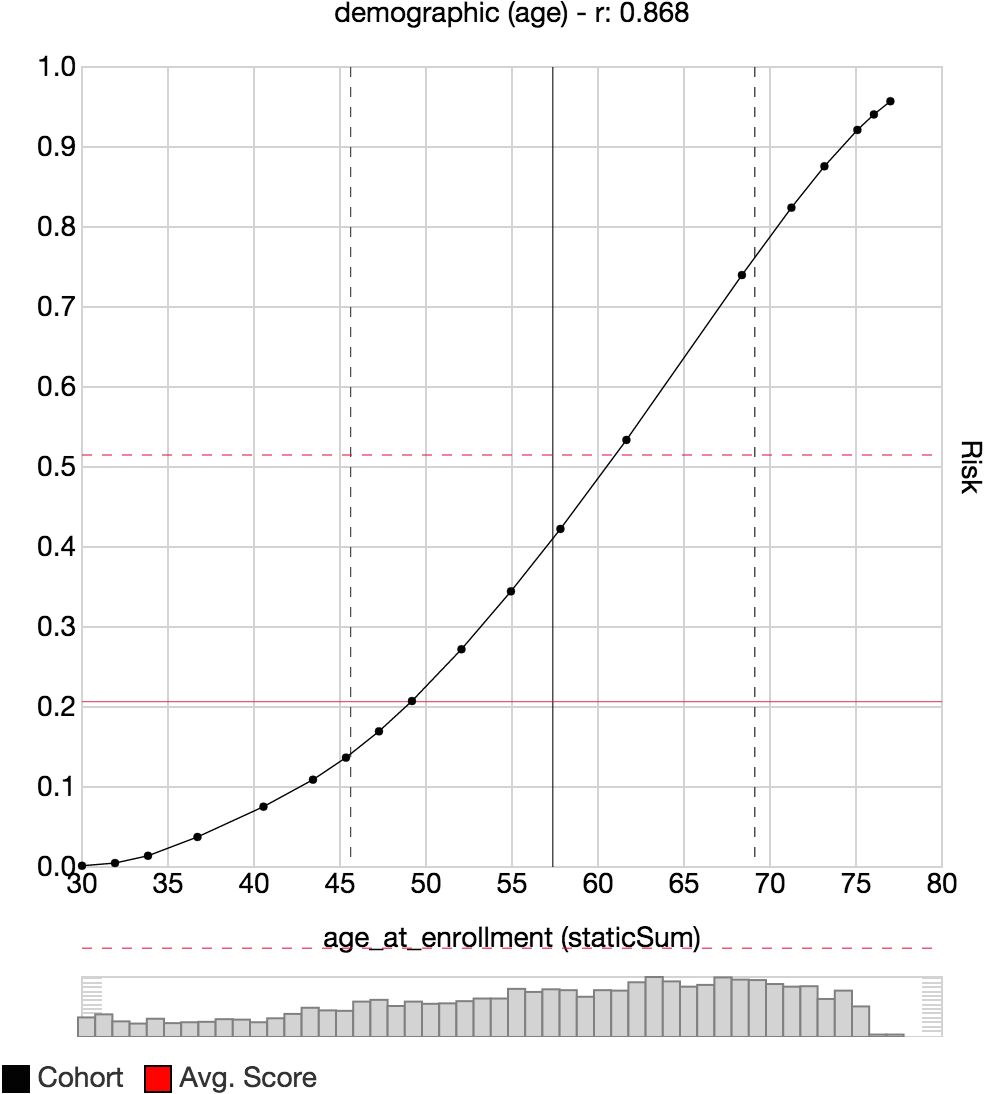
\includegraphics[width=0.6\linewidth]{prospector/pdp_reg} % 0.7
\caption{
Partial dependence plots. The black curve shows the average predicted risk
(probability of a certain outcome) if for all rows in the data the value of this
feature was the given value of the horizontal axis.
The red line shows the average predicted risk for the original data.
The vertical line shows the mean of the observed values and the histogram below the plot
shows the distribution of observed values.
Dotted lines show the range of one standard deviation around the mean values.
}
\label{figs:pdp}
\end{figure}